\section{Evaluation}
\label{evaluation}

The following section will provide an evaluation of the two schemes based on an automated benchmark implemented as part of the C++ library described in the previous section. The benchmark measures the following metrics of each LSH scheme:

\begin{itemize}
  \item \textbf{Insertion throughput:} How many items can be inserted into the data structure per second?
  \item \textbf{Query throughput:} How many queries can be performed against the data structure per second?
  \item \textbf{Bucket distribution:} How efficiently does the scheme distribute items in buckets across partitions?
  \item \textbf{False negative rate:} How many false negatives occur per query?
\end{itemize}

The benchmark performs a 1-NN search in each of three configured tables: A brute force table, a classic table, and a covering table. The purpose of the brute force table is to establish the ground truth by locating the exact nearest neighbour for each of the query items. This ground truth is then used for determining if a false negative has been encountered for each of the query results in the classic and covering tables.

\paragraph{Dataset} The dataset used for the evaluation is a pre-processed version of the \texttt{ANN\_SIFT1M} set distributed as part of the Multi Index Hashing (MIH) library located at \url{https://github.com/norouzi/mih}.

This dataset is created specifically for the evaluation of approximate nearest neighbour search algorithms and is a set of 1 million image feature vectors of 128 dimensions, plus an additional 10,000 query vectors. The version distributed alongside the MIH library is however binarized to vectors of 64 dimensions using LSH, which better suits the purpose of our evaluation.

\paragraph{Parameters} Our choice of parameters follows that of the experiments carried out in \cite{DBLP:journals/corr/PhamP16}. That is, for a given radius $r$, we set the number of partitions to use in the classic table to $l = 2^{r + 1} - 1$ and the number of bits to sample to $k = 􏰢\frac{\log(1 - \delta^{1 / l})}{\log(1 - \frac{r}{d})}$.􏰣 For the covering table we just need the radius $r$.

\subsection{Results}

The results were obtained by running the benchmark on a 2.8 GHz Intel Core i5 processor with a 3 MB L3 cache and 8 GB of DDR3 memory. Due to the limited amount of memory available, we have only been able to provide results for $r \in \{2,\ldots,5\}$.

\subsubsection{Insertions per second}

Figure ~\ref{fig:insertions-per-second} presents how many insertions per second are performed. As we assumed and can conclude from figure XX  Covering LSH has lowest performance due need of construction additional buckets. But the gap between Covering LSH and the regular ones is relatively small and by the radius is increasing we can actually see that the result are coming closer. At the radius of 5 the difference is almost 3 times smaller than at the initial radius of 2. By increasing radius the classic LSH is forced to produce more buckets so one the insertion time increases.

\begin{figure}[ht]
    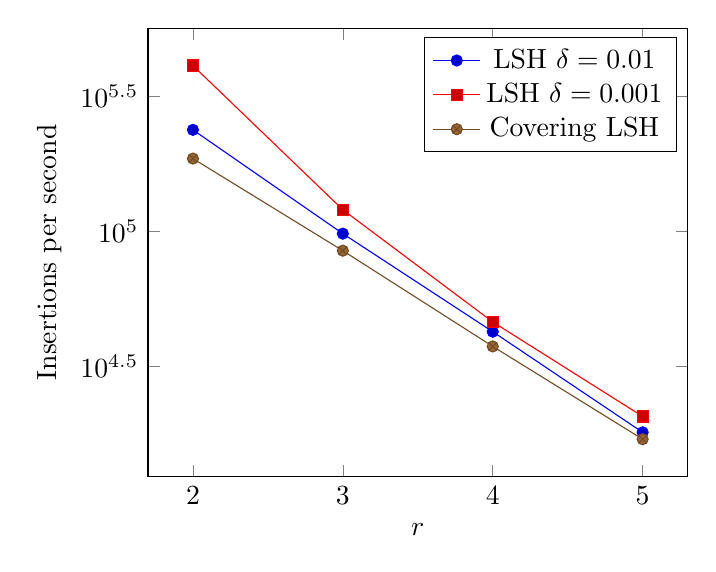
\begin{tikzpicture}
    \begin{semilogyaxis}[
      xlabel = {$r$},
      ylabel = {Insertions per second},
      xtick = data
    ]
      \addplot coordinates {
        (2, 237736.94)
        (3, 98187.51)
        (4, 42593.97)
        (5, 18074.10)
      };

      \addplot coordinates {
        (2, 411106.15)
        (3, 120359.67)
        (4, 46280.57)
        (5, 20693.81)
      };

      \addplot coordinates {
        (2, 186131.05)
        (3, 84934.71)
        (4, 37573.59)
        (5, 17047.07)
      };

      \legend{LSH $\delta = 0.01$, LSH $\delta = 0.001$, Covering LSH}
    \end{semilogyaxis}
  \end{tikzpicture}

  \caption{Comparision of insertion throughput}
  \label{fig:insertions-per-second}
\end{figure}

\subsubsection{Queries per second}

Figure ~\ref{fig:queries-per-second} presents throughput of each LSH. By the problem definition we were suspecting that the Covering LSH trade off performance for guarantee of producing results begin free of false negatives. The result are rather surprising. Throughput of the Covering LSH is actually outclassing the Classic LSH. As far the radius comes one the performance drops but still maintains advantage over the Classic ones. By the current range of results we can expect that it scales better - trend of Covering and Classic $\delta = 0.001$ looks very similar but still the throughput of Covering is twice better.

\begin{figure}[ht]
  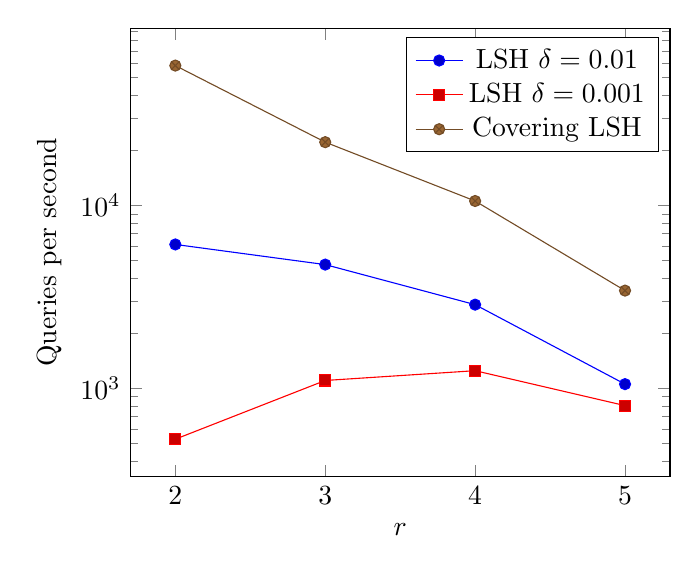
\begin{tikzpicture}
    \begin{semilogyaxis}[
      xlabel = {$r$},
      ylabel = {Queries per second},
      xtick = data
    ]
      \addplot coordinates {
        (2, 6118.88)
        (3, 4747.76)
        (4, 2866.80)
        (5, 1053.48)
      };

      \addplot coordinates {
        (2, 526.67)
        (3, 1103.17)
        (4, 1247.75)
        (5, 803.80)
      };

      \addplot coordinates {
        (2, 58216.55)
        (3, 22187.94)
        (4, 10574.71)
        (5, 3421.63)
      };

      \legend{LSH $\delta = 0.01$, LSH $\delta = 0.001$, Covering LSH}
    \end{semilogyaxis}
  \end{tikzpicture}

  \caption{Comparision of query throughput}
  \label{fig:queries-per-second}
\end{figure}

\subsubsection{Buckets per partition}

Figure ~\ref{fig:buckets-per-partition} presents how many buckets per partition is created. This metric show how much Covering LSH differs from the classic one. Amount of buckets in classic implementations is dependent on the radius. Where the Covering is totally opposite - the buckets count is constant. It is connected to the way how the hash functions family are created [reference]. The trend presented on the plot is very similar to the one from figure ~\ref{fig:insertions-per-second}. Again by increasing the radius the gap is closing. But still the memory overhead is significantly bigger in the Covering that in classic LSH.

\begin{figure}[ht]
  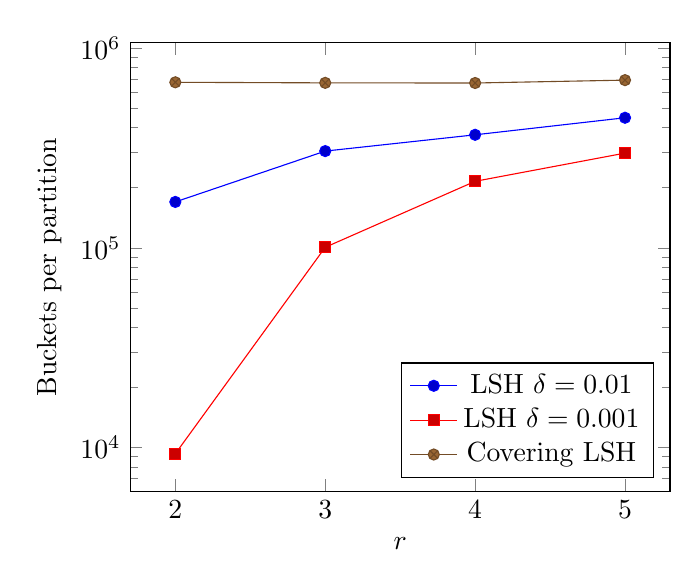
\begin{tikzpicture}
    \begin{semilogyaxis}[
      xlabel = {$r$},
      ylabel = {Buckets per partition},
      xtick = data,
      legend pos = south east
    ]
      \addplot coordinates {
        (2, 169815.43)
        (3, 305179.47)
        (4, 368261.81)
        (5, 448140.33)
      };

      \addplot coordinates {
        (2, 9310.57)
        (3, 100652.33)
        (4, 215357.87)
        (5, 298153.22)
      };

      \addplot coordinates {
        (2, 674554.00)
        (3, 670221.60)
        (4, 669083.68)
        (5, 691636.11)
      };

      \legend{LSH $\delta = 0.01$, LSH $\delta = 0.001$, Covering LSH}
    \end{semilogyaxis}
  \end{tikzpicture}

  \caption{Comparision of bucket distribution}
  \label{fig:buckets-per-partition}
\end{figure}

\subsubsection{False negatives per query}

The most important property of the Covering LSH is the fact that it guartees that the queries are not producing false negatives. Figure ~\ref{fig:false-negatives-per-query} show the comparision of this metric between implementations. Obviously the covering holds zero false negatives in each case. More surprising are the results of the classic LSH. Especially the $\delta = 0.001$ presents very low amount of false negatives across the cases. Next classic LSH is far worse than that; it has more false negatives in each case of $r$.

\begin{figure}[ht]
  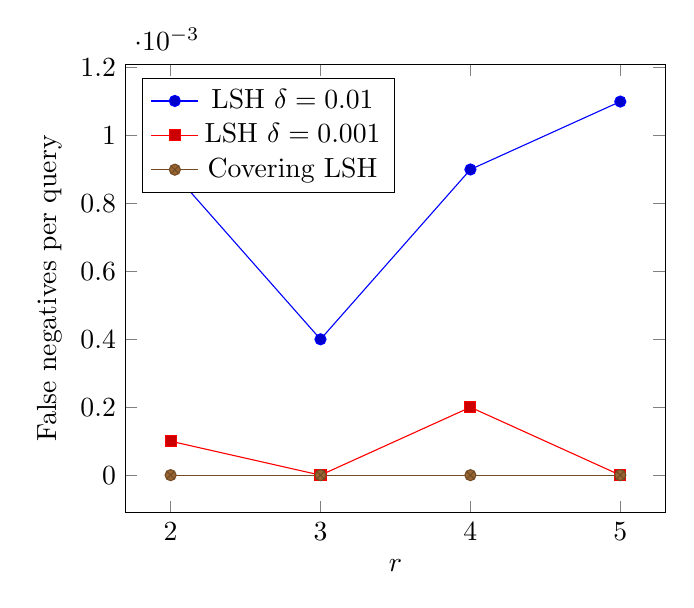
\begin{tikzpicture}
    \begin{axis}[
      xlabel = {$r$},
      ylabel = {False negatives per query},
      xtick = data,
      legend pos = north west
    ]
      \addplot coordinates {
        (2, 0.0009)
        (3, 0.0004)
        (4, 0.0009)
        (5, 0.0011)
      };

      \addplot coordinates {
        (2, 0.0001)
        (3, 0.0000)
        (4, 0.0002)
        (5, 0.0000)
      };

      \addplot coordinates {
        (2, 0.0000)
        (3, 0.0000)
        (4, 0.0000)
        (5, 0.0000)
      };

      \legend{LSH $\delta = 0.01$, LSH $\delta = 0.001$, Covering LSH}
    \end{axis}
  \end{tikzpicture}

  \caption{Comparison of false negative rates}
  \label{fig:false-negatives-per-query}
\end{figure}
